% % % % % % % % % % % % % % % % % % % % % % % % % % % % % % % % % % % % % % % %
\section{Pár úvodných slov}

Začneme typickým príkladom, ktorý sa v tej či onej modifikácii objaví v každom
texte o lineárnom programovaní.  Zoberme si študenta, ktorý na prípravu na
skúšku potrebuje dostať do tela aspoň $270$~mg kofeínu a $120$~g cukru.
Zároveň nechce prekročiť dávku $180$~mg aspartámu. K dispozícii má dva nápoje:
hnedú vodu za \hbox{\EUR{$1$}/dl} a zelenú vodu za \hbox{\EUR{$1,50$}/dl.}
Hnedá voda obsahuje $30$~mg kofeínu, $40$~g cukru a $40$~mg aspartámu, kým
zelená voda obsahuje $90$~mg kofeínu, $30$~g cukru a $30$~mg aspartámu. Koľko dl
ktorej vody si má študent kúpiť, aby čo najlacnejšie uspokojil svoje
požiadavky? Ak si študent kúpi $x$~dl hnedej vody a $y$~dl zelenej vody, úlohu
(nazývanú {\em lineárny program}) môžme formulovať takto:

\begin{equation}
  \label{eq:LP:1}
\begin{array}{rccccll}
                          & \multicolumn{3}{c}{\text{dl vody}} \\ 
                          & \text{hnedej} & & \text{zelenej}\\
  \text{minimalizovať}     & x   & + & 1.5 y & =: & f(x,y) &  \text{\em cena}\\
   {\rm pri\ obmedzeniach} & \color{blue}{30 x } & \color{blue}{+} & \color{blue}{90 y} & \color{blue}{\ge} & \color{blue}{270} & \text{\color{blue}{\em kofeín}}\\ 
                           & \color{red}{40 x}   & \color{red}{+}  & \color{red}{30 y}  & \color{red}{\ge} & \color{red}{120} & \text{\color{red}{\em cukor}} \\
                           & \color{magenta}{40 x} & \color{magenta}{+} & \color{magenta}{30 y} & \color{magenta}{\le} & \color{magenta}{180} & \text{\color{magenta}{\em aspartám}}\\
                          &      &   & x,y  &\ge& 0
\end{array}
\end{equation}
%
Ľahko vidno, že napr. 4~dl zelenej vody uspokoja všetky požiadavky za cenu
\EUR{6}, pričom kofeínu je aj viac, ako je nutné a aspartámu menej, ako je
dovolené. Na druhej strane, ak by študent chcel kupovať iba hnedú vodu, na
splnenie potreby kofeínu by jej musel kúpiť 9~dl, čím by ale prekročil
prípustný príjem aspartámu (a navyše by to bolo drahé). Pri hľadaní optimálneho
riešenia pomôže nasledovná geometrická reprezentácia: ak riešeniu s $x$~dl
hnedej a $y$~dl zelenej vody priradíme bod v rovine so súradnicami $(x,y)$,
každé z obmedzení určuje polrovinu, v ktorej prípustné riešenie musí ležať.
Do úvahy preto prichádzajú iba riešenia v štvoruholníku z ľavého obrázka:


% draws a halfplane
% optional: paameters to draw
% fist point, second point, orientation (+/-), length1, length2
\shorthandoff{-}
\newcommand{\halfplane}[6][ ]{%
  \coordinate (O) at (#2);
  \coordinate (XX) at (#3);
  \coordinate (YY) at ($ (O) !1! 90:(XX) $);
  \coordinate (X) at ($ (XX) - (O) $);
  \coordinate (Y) at ($ (YY) - (O) $);
  \coordinate (E) at ($ (XX)!#6! ($(XX)+(X)$) $);
  \begin{scope}[#1]
      \draw 
          ($ (O)!-#5!(XX) $) -- (E);
     
      \foreach \i in {0,0.1,...,1}  
          \draw
          let
              \p1 = ($ ($ (E) !1.5cm! (O) $) + ($ (0,0) !\i cm! (X) $) $)
         in
              (\p1) -- ($ (\p1) ! 8pt ! #4 330:($ (\p1)+($ (0,0)#4(Y) $) $) $);
  \end{scope}
}

\renewcommand{\common}{%
  %axis
  \draw (-2,0) -- coordinate (x axis mid) (11,0);
  \draw (0,-2) -- coordinate (y axis mid) (0,8);
  %ticks
  \foreach \x in {-2,...,10}
      \draw (\x,1pt) -- (\x,-3pt);
  \foreach \x in {2,4,...,10}
      \draw (\x,-3pt) node[anchor=north] {\x};
  \foreach \y in {1,...,7}
      \draw (1pt,\y) -- (-3pt,\y) 
          node[anchor=east] {\y}; 
      \draw (0,0) node[anchor=north east]{$0$};
  %labels      
  \node[below=0.8cm] at (x axis mid) {hnedá voda};
  \node[rotate=90] at (-2,4) {zelená voda};
  
  \filldraw[fill=black!50, line width=0.8pt, fill opacity=0.5 ]
    (0,6) -- (0,4) -- (1,2.66) -- (3,2) -- cycle;
}


\begin{center}
\begin{tikzpicture}[scale=0.5]
  \halfplane[color=red]{0,4}{3,0}{+}{1cm}{1cm}
  \halfplane[color=blue]{9,0}{0,3}{-}{1cm}{1cm}
  \halfplane[color=magenta]{0,6}{4.5,0}{-}{1cm}{1cm}

  \common
\end{tikzpicture}
\hfill
\begin{tikzpicture}[scale=0.5]
  \begin{scope}
    \clip (-1,-0.4) -- (11,-0.4) -- (11,8) -- (-1,8) -- cycle;
    \coordinate (v) at (3,-2);
    \draw[dashed,color=black!80]  
        \foreach \p in {(1,2.66),(0,4),(0,6),(0,7)}
            {($ (\p ! 20cm ! ($ (\p - (v) $) $)  -- ($ (\p ! 20cm ! ($ (\p + (v) $) $)};
    \coordinate (q) at ($ (0,7) !4cm! ($ (0,7) + (v) $) $);
    \draw[thick,->]
        (5,6) node[anchor=south west] {$f(x,y)=10.5$}  -- (q) ;
  \end{scope}
  
      
  \common
  \filldraw[very thin,red,dotted]
        (1,2.66) circle (2pt) -- (0,2.66)
        (1, 2.66) -- (1,0);
\end{tikzpicture}
\end{center}
%
Zároveň vieme, že $f(x,y)=x+1.5y$ je lineárna funkcia, a preto body s rovnakou
hodnotou funkcie $f$ ležia na priamke (viď. pravý obrázok). Preto je zrejmé, že
stačí overiť štyri vrcholy štvoruholníka a nájdeme optimálne riešenie, ktoré je
v tomto prípade kúpiť 1~dl hnedej vody a $2\frac{2}{3}$~dl zelenej vody za  \EUR{5}.

\noindent
\begin{minipage}[t]{\textwidth-6cm}
\vspace{0pt}
Z týchto úvah ľahko odvodíme algoritmus na riešenie úlohy s dvoma premennými a
obmedzeniami s nerovnosťami: pre každé obmedzenie zostrojíme príslušnú
polrovinu, skonštruujeme mnohouholník, ktorý je prienikom všetkých polrovín a
vyberieme optimálnu hodnotu spomedzi jeho vrcholov.  Pre tri premenné
obmedzenia tvaru $a_1x+a_2y+a_3z\ge b$ tvoria polpriestory, ktorých prienikom
dostaneme mnohosten. Body s rovnakou hodnotou funkcie $f(x,y,z)=c_1x+c_2y+c_3z$
tvoria rovinu a preto na nájdenie optima stačí overiť všetky vrcholy
mnohostena.\\
\end{minipage}
\begin{minipage}[t]{6cm}
  \vspace{0pt}
  % origin, side (vector), second side
\newcommand{\kvad}[3]{%
    (#1) -- ($ (#1) + (#2) $) -- ($ (#1) + (#2) + (#3) $) -- ($ (#1) + (#3) $) -- cycle
}

% new_point_name x y z  (RotatedOriginShift should be set)
\newcommand{\rottomain}[4]{
    \tdplottransformrotmain{#2}{#3}{#4}
    \coordinate (#1) at ($ (\tdplotresx,\tdplotresy,\tdplotresz) + (RotatedOriginShift) $);
}

% intersection of two lines: name and four endpoints
\newcommand{\intersect}[5]{
    \path [name path=intersect_p1] (#2) -- (#3);
    \path [name path=intersect_p2] (#4) -- (#5);
    \path [name intersections={of=intersect_p1 and intersect_p2, by={#1}} ];
}

\renewcommand{\axes}{%
    \draw[thick,->] 
      (0,0,0) -- (1.3,0,0) node[anchor=north east]{$x$}
      (0,0,0) -- (0,1.3,0) node[anchor=north west]{$y$}
      (0,0,0) -- (0,0,1.3) node[anchor=south]{$z$};
    \draw[thick,->,tdplot_rotated_coords,color=blue] 
      (0,0,0) -- (1,0,0) node[anchor=north east]{$x$}
      (0,0,0) -- (0,1,0) node[anchor=north west]{$y$}
      (0,0,0) -- (0,0,1) node[anchor=south]{$z$};
}

\begin{center}
  \tdplotsetmaincoords{70}{60}
  \begin{tikzpicture}[scale=2,tdplot_main_coords]

    \tdplotsetrotatedcoords{45}{55}{5}    
    \coordinate (RotatedOriginShift) at (1,1,1);
    \tdplotsetrotatedcoordsorigin{(RotatedOriginShift)}
    %\axes       

    \fill[fill=black!30,fill opacity=0.3]
        \kvad{0,0,0}{1,0,0}{0,1,0}
        \kvad{0,0,0}{0,1,0}{0,0,1}
        \kvad{1,1,1}{-1,0,0}{0,0,-1}
        \kvad{1,1,1}{0,-1,0}{0,0,-1};
    \fill[fill=black!90, fill opacity=0.3]
        \kvad{0,0,0}{1,0,0}{0,0,1};
    \fill[fill=black!50, fill opacity=0.3]
        \kvad{0,0,1}{1,0,0}{0,1,0};
        

  
    % blue kvad  
    \rottomain{p1}{-0.7}{-1}{0} % origin
    \rottomain{p2}{0.7}{-1}{0}  % o + x
    \rottomain{p3}{-0.7}{1}{0}  % o + y

    \intersect{i1}{p1}{p2}{1,0,1}{1,1,1}
    \intersect{i2}{p1}{p3}{0,0,1}{0,1,1}
    \intersect{i3}{p1}{p2}{1,1,0}{1,1,1}

    \draw
        (1,0,1) -- (i1)
        (0,0,1) -- (i2)
        (1,1,0) -- (i3)
        \kvad{0,0,0}{1,0,0}{0,0,1}
        (1,0,0) -- (1,1,0);

    \draw[dashed]    
        (i1) -- (1,1,1)
        (0,1,0) -- (1,1,0)
        (0,1,0) -- (0,0,0)
        (0,1,0) -- (0,1,1)
        (i2) -- (0,1,1)
        (i3) -- (1,1,1)
        (0,1,1) -- (1,1,1);

    \begin{scope}[tdplot_rotated_coords]
       \filldraw[color=blue,very thin,fill=blue!20,fill opacity=0.5]
          \kvad{-0.7,-1,0}{1.4,0,0}{0,2,0};
        %\draw[color=blue,very thick,->]  
        %  (0,0,0) -- (0,0,1);
        \fill[color=blue]
          (0,0,0) circle (1pt);
    \end{scope}


  \end{tikzpicture}
\end{center}

\end{minipage}


\noindent S narastajúcim počtom premenných začnú rásť aj problémy a je zrejmé,
že priamočiarym zovšeobecňovaním sa ďaleko nedostaneme. Skúsme sa preto pozrieť
na geometriu lineárneho programu trochu inak.  Najprv si upravme program
(\ref{eq:LP:1}) do ekvivalentnej podoby takto: funkciu $f(x,y)$ vynásobíme -1 a
z minimalizačnej úlohy dostaneme maximalizačnú. Potom prvé a druhé obmedzenie
vynásobíme -1 a všetky obmedzenia (okrem tých na nezápornosť $x,y$) budú v
tvare ``$\le$''. Nakoniec, keďže v každom obmedzení je ľavá strana menšia ako
pravá, môžme pridať novú nezápornú premennú, ktorej hodnota bude práve rozdiel
ľavej a pravej strany a dostaneme nasledujúci program, ktorý je očividne
ekvivalentný s pôvodným.


\begin{equation}
\label{eq:LP:2}
\begin{array}{rrrrrrcl}
  \text{maximalizovať}     & -x   & -  1.5y &         &         &       & =: & f(x,y,s_1,s_2,s_3) \\
   {\rm pri\ obmedzeniach}& -30x & -  90y  & +   s_1 &         &       & =  & -270\\
                          & -40x & -  30y  &         & +   s_2 &       & =  & -120\\
                          &  40x & +  30y  &         &         &+  s_3 & =  & 180\\      
                          &      &         &     \multicolumn{3}{r}{x,y,s_1,s_2,s_3}  &\ge& 0
\end{array}
\end{equation}
%
Ak si označíme
\begin{align*}
 \bm{c}&=\cvect{-1\\-1.5\\0\\0\\0}
&A&=\left(\begin{array}{ccccc}-30&-90&1&0&0\\-40&-30&0&1&0\\30&40&0&0&1\end{array}\right)
&\bm{b}&=\cvect{-270\\-120\\200}
\end{align*}
tak program (\ref{eq:LP:2}) môžeme skrátene zapísať
$$\max_{\bm{x}\in\R^5}\left\{ \bm{c}\tr\bm{x} \mid A\bm{x}=\bm{b},\; \bm{x}\ge0
\right\}.$$ Týmto prepísaním sme zvýšili dimenziu problému z 2 na 5 (a tak sme
stratili možnosť ``obrázkového'' riešenia), ale získali sme krajší tvar množiny
prípustných riešení: sú to nezáporné riešenia systému lineárnych rovníc.  V
našom prípade má matica $A$ hodnosť 3 (riadky sú lineárne nezávislé) a riešenia
systému $A\bm{x}=\bm{b}$ tvoria dvojrozmerný podpriestor
$\bm{o}+c_1\bm{\alpha}+c_2\bm{\beta}$ kde
\begin{align*}
\bm{o}&=\cvect{0\\0\\-270\\-120\\180}
      &\bm{\alpha}&=\cvect{1\\0\\30\\40\\-40}
      &\bm{\beta}&=\cvect{0\\1\\90\\30\\-30}.
\end{align*}
Inými slovami, prípustné riešenia programu (\ref{eq:LP:1}) tvoria 2-rozmerný
útvar (štvoruholník) v dvojrozmernom priestore (rovine), kým prípustné riešenia
programu (\ref{eq:LP:2}) tvoria 2-rozmerný útvar \dom v 5-rozmernom priestore,
pričom \dom je prienikom (2-rozmernej) roviny a kladného ortantu\footnote{ako
  je kvadrant v rovine a oktant v 3D priestore, používame slovo ortant v
$n$-rozmernom priestore}. Pre ilustráciu uvažujme nasledovné jednoduchšie
programy (uvádzame iba obmedzenia, na účelovej funkcii v tomto prípade
nezáleží):


\renewcommand{\commonii}{%
  %axis
  \draw (-0.5,0) -- coordinate (x axis mid) (1.5,0);
  \draw (0,-0.2) -- coordinate (y axis mid) (0,1.5);
  %ticks
  \foreach \x in {-0.2,-0.1,...,1.4}
      \draw (\x,1pt) -- (\x,-3pt);
  \draw (1,-3pt) node[anchor=north] {1};

  \foreach \y in {0.2,0.3,...,1.4}
      \draw (1pt,\y) -- (-3pt,\y);
  \draw (-1pt,1) node[anchor=east] {1}; 
  
  \draw (0,-3pt) node[anchor=north east]{$0$};
}


\renewcommand{\axes}{
    \draw
      (0,0,0) -- (1.5,0,0) node[anchor=north east]{$x$}
      (0,0,0) -- (0,1.5,0) node[anchor=north west]{$y$}
      (0,0,0) -- (0,0,1.5) node[anchor=south]{$s$};
}


\setlength{\picx}{(0.5\textwidth - 3cm)/2}
\setlength{\picy}{\picx}
\begin{tikzpicture}[x=\picx,y=\picy]
  \fill[fill=blue!50, opacity=0.8]
    (0,0) -- (1,0) -- (0,1) -- cycle;
  \commonii
  \draw[thick, shorten >= -10pt, shorten <= -10pt] (0,1) -- (1,0);
  \draw (0.7,1) node {$\begin{array}{rl}x+y&\le 1\\ x,y&\ge0\end{array}$};
  \foreach \p in {(0,0),(1,0),(0,1)}
    \filldraw \p circle (1.5pt); 
\end{tikzpicture}
\hfill
\tdplotsetmaincoords{70}{120}
\begin{tikzpicture}[scale=2.3,tdplot_main_coords]
  \axes
  \coordinate (u) at ($ (0,0,0)!2.5cm!(-1,1,0) $);
  \coordinate (v) at ($ (0,0,0)!2cm!(-1,-1,2) $);
  \coordinate (p) at ($ (1,0,0)!7mm! ($ (1,0,0)-($(u)+(v)$) $) $);
  
  \filldraw[fill=blue!30, opacity=0.3]
      (p) -- ($ (p) + (u) $) -- ($ (p) + (u) + (v) $) -- ($ (p) + (v) $) -- cycle;
  \draw[thin]
      (p) -- ($ (p) + (u) $) -- ($ (p) + (u) + (v) $) -- ($ (p) + (v) $) -- cycle;

  \filldraw[thick,fill=blue!50, opacity=0.8]
      (1,0,0) -- (0,1,0) -- (0,0,1) -- cycle;
  \foreach \p in {(1,0,0),(0,1,0),(0,0,1)}
    \filldraw \p circle (.8pt); 
 
   \draw[tdplot_screen_coords] (0.7,1) node {$\begin{array}{rl}x+y+s&= 1\\ x,y,s&\ge0\end{array}$};

\end{tikzpicture}

\noindent Vľavo je program s dvoma premennými a dvojrozmerným priestorom
riešení. Po transformácii do troch rozmerov priestor riešení ostal dvojrozmerný
útvar a je  prienikom roviny a kladného oktantu. V nasledujúcom prípade je v
pôvodnom probléme priestor riešení jednorozmerný; po transformácii do
trojrozmerného priestoru je priestor riešení stále jednorozmerný a je prienikom
priamky a kladného oktantu. 

\begin{tikzpicture}[x=\picx,y=\picy]
  \fill[fill=blue!30, opacity=0.3]
    (0,0) -- (1,0) -- (0,1) -- cycle;
  \draw[shorten >= -2cm, shorten <= -3pt] (0,0) -- (.5,.5);
  \draw[very thick]
    (0,0) -- (0.5,0.5);
  \commonii
  \draw[shorten >= -10pt, shorten <= -10pt] (0,1) -- (1,0);

  \draw (0.6,1.5) node {$\begin{array}{rl}x+y&\le 1\\ x-y&=0\\x,y&\ge0\end{array}$};
  \foreach \p in {(0,0),(.5,.5)}
    \filldraw \p circle (1.5pt); 
\end{tikzpicture}
\hfill
\tdplotsetmaincoords{70}{120}
\begin{tikzpicture}[scale=2.3,tdplot_main_coords]
  \axes
  \coordinate (u) at ($ (0,0,0)!2.5cm!(-1,1,0) $);
  \coordinate (v) at ($ (0,0,0)!2cm!(-1,-1,2) $);
  \coordinate (p) at ($ (1,0,0)!7mm! ($ (1,0,0)-($(u)+(v)$) $) $);
  
  \filldraw[fill=blue!30, opacity=0.3]
      (p) -- ($ (p) + (u) $) -- ($ (p) + (u) + (v) $) -- ($ (p) + (v) $) -- cycle;
  \draw[thin]
      (p) -- ($ (p) + (u) $) -- ($ (p) + (u) + (v) $) -- ($ (p) + (v) $) -- cycle;

  \coordinate (u) at ($ (0,0,0)!1cm!(1,1,0) $);
  \coordinate (v) at ($ (0,0,0)!1.8cm!(0,0,1) $);
  \coordinate (p) at ($ (0,0,0)!3mm! ($ (0,0,0)-($(u)+(v)$) $) $);
  
  \filldraw[fill=green!30, opacity=0.3]
      (p) -- ($ (p) + (u) $) -- ($ (p) + (u) + (v) $) -- ($ (p) + (v) $) -- cycle;
  \draw[thin]
      (p) -- ($ (p) + (u) $) -- ($ (p) + (u) + (v) $) -- ($ (p) + (v) $) -- cycle;
  

  \filldraw[color=blue!60, fill=blue!50, opacity=0.5]
      (1,0,0) -- (0,1,0) -- (0,0,1) -- cycle;
  \filldraw[color=green!60, fill=green!50, opacity=0.5]
      (0,0,0) -- (0,0,1) -- (.5,.5,0) -- cycle;


  \foreach \p in {(0,0,1),(.5,.5,0)}
    \filldraw \p circle (.8pt); 
 
  \draw[tdplot_screen_coords] (0.7,1.05) node {$\begin{array}{rl}x+y+s&=1\\ x-y&=0\\x,y,s&\ge0\end{array}$};
  \draw[very thin, dashed] 
      (0,0,0) -- (1.5,1.5,0)
      (0,0,0) -- (0,0,1)
      (1,0,0) -- (0,1,0) -- (0,0,1) -- cycle;
  \draw[very thick]
    (0,0,1) -- (0.5,0.5,0);

\end{tikzpicture}

\noindent Výhoda takto zapísaného programu je v tom, že sa nám budú ľahšie
hľadať vrcholy telesa prípustných riešení: budú určite ležať v nejakej stene
tvaru $x_i=0$.

Skôr, ako pokročíme v našich úvahách je dobré si uvedomiť, že bez ujmy na
všeobecnosti môžme predpokladať, že riadky  matice $A$ sú lineárne nezávislé:
ak je nejaký riadok lineárnou kombináciou iných riadkov potom buď neexistuje
žiadne prípustné riešenie, alebo jeho odstránením nijak nezmeníme priestor
prípustných riešení.  Naše úvahy môžme zhrnúť a zaviesť {\em normálny tvar}
lineárneho programu takto:

\vskip 1em
\noindent
\begin{framed}
  \begin{dfn}
  \label{df:LP:eqnormalform}
  Lineárny program je v {\bf normálnom tvare}, ak je zapísaný ako
\begin{equation}
  \max_{\bm{x}\in\R^n}\left\{ \bm{c}\tr\bm{x} \mid A\bm{x}=\bm{b},\;\bm{x}\ge\bm{0}\right\},
\end{equation}
kde $A\in\R^{m\times n}$ má hodnosť $m$. Množina prípustných hodnôt $\dom=\left\{\bm{x}\in\R^n \mid  A\bm{x}=\bm{b},\;\bm{x}\ge\bm{0}\right\}$.
\end{dfn}
\end{framed}

\begin{itemize}
\item {\bf Cieľom je maximalizácia.} Ak bolo pôvodným cieľom minimalizovať
lineárnu funkciu $f(\bm{x})$, novým cieľom bude maximalizovať lineárnu funkciu
$-f(\bm{x})$.
\item {\bf Všetky premenné sú nezáporné.} Pre každú premennú $x$, ktorá nemá obmedzenie $x\ge0$
pridáme dve premenné $p_x,q_x\ge0$ a každý výskyt $x$ nahradíme $p_x-q_x$.
\item {\bf Každé obmedzenie okrem tých tvaru $x\ge0$  má tvar rovnosti.} Ak
bolo pôvodné obmedzenie v tvare $\sum_ia_ix_i\ge b$, najprv ho prenásobením
$-1$ upravíme na tvar $\sum_i-a_ix_i\le-b$.  Keď máme všetky nerovnosti v
obmedzeniach otočené rovnakým smerom, pre každé obmedzenie tvaru
$\sum_ia_ix_i\le b$ zavedieme novú premennú $s$ ({\em rezerva, slack}), ktorá
reprezentuje hodnotu, o koľko je pôvodná ľavá strana menšia ako $b$. Ľahko
vidno, že $s\ge 0$ a $s+\sum_ia_ix_i=b$.  
\item {\bf Matica \bm{A} má \bm{m} lineárne nezávislých riadkov.}
\end{itemize} 

\noindent Majme teraz program v normálnom tvare. Podobne ako v úvodnom
príklade, chceme nájsť množinu vrcholov telesa \dom ohraničujúceho prípustné
riešenia tak, aby stačilo overiť tieto vrcholy na nájdenie optimálneho riešenia.
Keďže \dom je prienikom priestoru riešení $A\bm{x}=\bm{b}$ a kladného ortantu,
vrcholy budú mať jednu alebo niekoľko súradníc $x_{i_1},\ldots,x_{i_k}$ nulových
(nadrovina $x_i=0$ je na hranici ortantu).  Navyše, vrcholy sú ``špicaté'' (na
rozdiel od bodov v nejakej stene $x_i=0$, v ktorej leží napr. celá úsečka).
To, že vrchol je ``špicatý'', formulujeme tak, že ak k obmedzeniam  $A\bm{x}=\bm{b}$
pridáme navyše $x_{i_1}=0,\ldots,x_{i_k}=0$, dostaneme jednoznačné riešenie
(t.j. vrchol leží na prieniku nejakých stien ortantu a žiaden iný bod v tom istom
prieniku neleží).  Keďže $A$ má hodnosť $m$, na to, aby sme dostali jednoznačné
riešenie, musí byť $k=n-m$. 

\noindent Vráťme sa teraz k programu (\ref{eq:LP:2}).  Hodnosť matice $A$ je 3,
preto vrcholy dostaneme tak, že k systému $A\bm{x}=\bm{b}$ pridáme dve obmedzenia
$x_i=0$ a $x_j=0$.  Dostávame 10 rôznych systémov lineárnych rovníc s
nasledovnými riešeniami:

\vskip 1ex
{
\renewcommand{\arraystretch}{1.5}
\renewcommand{\tmp}[3]{\multicolumn{1}{#1>{\columncolor[gray]{0.9} $}#2<{$}#3}}

\noindent
\begin{minipage}[c]{6cm}
  \vskip 0pt
\begin{tabular}{|>{$}r<{$}|>{$}c<{$}>{$}c<{$}>{$}c<{$}>{$}c<{$}>{$}c<{$}|c}\cline{1-6}
    \text{obmedzenia}   & x   & y        & s_1 & s_2 & s_3  \\\cline{1-6}
  \rule{0mm}{3ex}                x=y=0  & 0     & 0          & -270  & -120  & 180  \\
                             x=s_1=0  & 0     & 3          & 0     & -30   & 90    \\
 \tmp{|}{r}{|}{x=s_2=0} & \tmp{}{c}{}{0}     & \tmp{}{c}{}{4}  & \tmp{}{c}{}{90}    &  \tmp{}{c}{}{0}    & \tmp{}{c}{|}{60} & A \\
 \tmp{|}{r}{|}{x=s_3=0} & \tmp{}{c}{}{0}     & \tmp{}{c}{}{6}  & \tmp{}{c}{}{270}   &  \tmp{}{c}{}{60}   & \tmp{}{c}{|}{0} & B\\
                y=s_1=0 & 9     & 0          & 0     &  240  &  -180 \\
                y=s_2=0 & 3     & 0          & -180  &  0    &  60\\
                y=s_3=0 & 4.5 & 0          & -135  &  60   &  0\\
 \tmp{|}{r}{|}{\bm{s_1=s_2=0}} & \tmp{}{c}{}{\bm{1}}     &\tmp{}{c}{}{\bm{\frac{8}{3}}} & \tmp{}{c}{}{\bm{0}}     &  \tmp{}{c}{}{\bm{0}}    &  \tmp{}{c}{|}{\bm{60}}& C\\
 \tmp{|}{r}{|}{s_1=s_3=0}      & \tmp{}{c}{}{3}     &\tmp{}{c}{}{2}           & \tmp{}{c}{}{0}     &  \tmp{}{c}{}{60}   &  \tmp{}{c}{|}{0} & D\\
                                  s_2=s_3=0&\multicolumn{5}{c|}{neexistuje riešenie}\\\cline{1-6}
  \end{tabular}
\end{minipage}
\hfill
\begin{minipage}[c]{5.6cm}
  \vskip 0pt
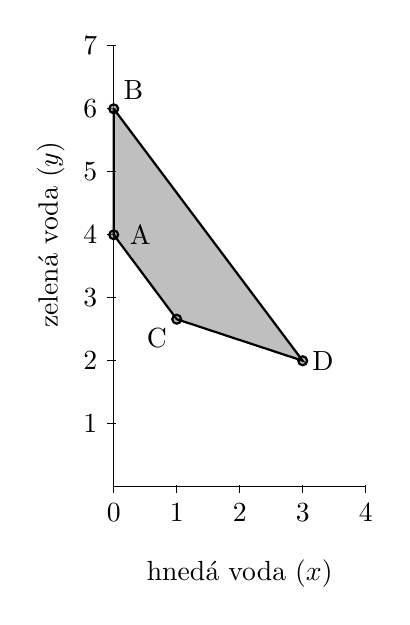
\begin{tikzpicture}[scale=0.8]
  %axis
  \draw (0,0) -- coordinate (x axis mid) (4,0);
  \draw (0,0) -- coordinate (y axis mid) (0,7);
  %ticks
  \foreach \x in {0,...,4}
      \draw (\x,1pt) -- (\x,-3pt);
  \foreach \x in {0,...,4}
      \draw (\x,-3pt) node[anchor=north] {\x};
  \foreach \y in {1,...,7}
      \draw (1pt,\y) -- (-3pt,\y) 
          node[anchor=east] {\y}; 
  %labels      
  \node[below=0.8cm] at (x axis mid) {hnedá voda ($x$)};
  \node[rotate=90] at (-1,4) {zelená voda ($y$)};
  
  \filldraw[fill=black!50, line width=0.8pt, fill opacity=0.5 ]
    (0,6) -- (0,4) -- (1,2.66) -- (3,2) -- (0,6)
    (0,6) circle (2pt)
    (0,4) circle (2pt)
    (1,2.66) circle (2pt)
    (3,2) circle (2pt);

    \draw (0,6) node[anchor=south west]{B};  
    \draw (.1,4) node[anchor=west]{A};  
    \draw (3,2) node[anchor=west]{D};  
    \draw (1,2.66) node[anchor=north east]{C};  
\end{tikzpicture}
\end{minipage}

}

\vskip 2ex
\noindent Riešenia systému $A\bm{x}=\bm{b}$ tvoria rovinu v 5-rozmernom
priestore. Premenné $x,y$ zodpovedajú množstvu kúpenej hnedej a zelenej vody,
premenné $s_1,s_2,s_3$ udávajú rezervu, ktorá ostáva k prekročeniu príslušného
obmedzenia. Takže napríklad štvrtý riadok tabuľky s obmedzeniami $x=s_3=0$
hovorí, že ak študent nekupuje žiadnu hnedú vodu a zároveň chce presne
dosiahnuť povolené množstvo aspartámu, musí kúpiť 6~dl zelenej vody, pričom
dostane viac kofeínu a cukru ako potrebuje. V poslednom riadku vidno, že
obmedzenia sa nedajú pridávať ľubovoľne, ale treba dávať pozor, aby pridaním
obmedzení nevznikli lineárne závislé riadky (v našom prípade sú červená a
fialová priamka z prvého obrázka rovnobežné, takže neexistuje žiaden bod v ich
priesečníku). V reči lineárnych programov sa riadkom tejto tabuľky hovorí {\em
bázové riešenia} a tie z nich, ktoré sú zároveň prípustné (zvýraznené riadky)
sú {\em prípustné bázové riešenia} a zodpovedajú vrcholom \dom, t.j. prípustné
riešenia programu (\ref{eq:LP:2}) tvoria dvojrozmerný štvoruholník v päťrozmernom
priestore.

\noindent
Za povšimnutie stojí, že prípustné bázové riešenia programu
(\ref{eq:LP:2}), t.j. vrcholy štvoruholníka prípustných riešení
v päťrozmernom priestore,  zodpovedajú vrcholom štvoruholníka prípustných riešení 
programu (\ref{eq:LP:1}): každý vrchol štvoruholníka vpravo leží na priesečníku dvoch priamok,
z ktorých každá zodpovedá obmedzeniu tvaru $x_i=0$ (a príslušné bázové riešenie
je prípustné). Naopak, každé prípustné bázové riešenie leží na priesečníku dvoch takýchto priamok.

\vskip 1ex
\noindent
Keď si uvedomíme,
že pridaním obmedzenia tvaru $x=0$ vlastne pri riešení príslušného systému
vymažeme stĺpec premennej $x$ z matice dostaneme nasledovnú definíciu.

\begin{ozn}
Majme maticu $A\in\R^{m\times n}$ s $m$ riadkami a $n$ stĺpcami. Pre množinu
$B\subseteq\{1,2,\ldots,n\}$ označíme $A_B$ podmaticu $A$, ktorá pozostáva zo
stĺpcov indexovaných množinou $B$. Rovnakú notáciu $\bm{x}_B$ budeme používať
pre vektory.
\end{ozn}

\noindent
Napríklad
\begin{align*}
A&=\left(\begin{array}{ccccc}-30&-90&1&0&0\\-40&-30&0&1&0\\30&40&0&0&1\end{array}\right)
 &A_{\{1,2\}}&=\left(\begin{array}{ccccc}-30&-90\\-40&-30\\30&40\end{array}\right)
 &A_{\{3,4,5\}}&=\left(\begin{array}{ccccc}1&0&0\\0&1&0\\0&0&1\end{array}\right)
\end{align*}


\begin{framed} 
  \begin{dfn} 
    \label{dfn:LP:basis} 
    Majme lineárny program v normálnom tvare, kde $A\in\R^{m\times n}$.
    {\bfseries Bázové riešenie} je vektor  $\bm{x}\in\R^n$, pre ktorý existuje
    $m$-prvková množina $B\subseteq\{1,\ldots,n\}$ taká, že
    \begin{enumerate}
      \item matica $A_B\in\R^{m\times m}$ má hodnosť $m$ (t.j. je regulárna)
      \item $x_j=0$ pre všetky $j\not\in B$
    \end{enumerate}
  \end{dfn}
\end{framed}

\noindent Teraz ukážeme, že naša predstava bázového riešenia ako vrchola je dobrá
v tom, že na nájdenie optima stačí overiť prípustné bázové riešenia.

\begin{veta}
Majme daný lineárny program v normálnom tvare, pričom hodnota
účelovej funkcie je $\bm{c}\tr\bm{x}$ na telese \dom je zhora ohraničená.
Potom pre každé prípustné riešenie $\bm{x_0}$ existuje prípustné bázové
riešenie $\bm{\tilde{x}}$, pre ktoré
$\bm{c}\tr\bm{\tilde{x}}\ge\bm{c}\tr\bm{x_0}$.
\end{veta}

\begin{dokaz}
Zoberme si ľubovoľné prípustné riešenie $\bm{x_0}$ a uvažujme všetky také
prípustné riešenia $\bm{x}$, pre ktoré $\bm{c}\tr\bm{x}\ge\bm{c}\tr\bm{x_0}$.
Za $\bm{\tilde{x}}$ vyberme také z nich, ktoré má najväčší počet nulových
zložiek.  Ukážeme, že $\bm{\tilde{x}}$ je bázové.  Ak $\bm{\tilde{x}}=\bm{0}$,
je zrejme bázové. Nech teda $\bm{\tilde{x}}$ má aspoň jednu nenulovú zložku.
Označme $K=\left\{j\in\{1,\ldots,n\}\mid\tilde{x}_j>0\right\}$ množinu kladných
(žiadne prípustné riešenie nemá záporné zložky) zložiek vektora
$\bm{\tilde{x}}$ a uvažujme dva prípady.

\bulpar {\em Stĺpce matice $A_K$ sú lineárne nezávislé.} Zjavne $|K|\le m$
(matica $A$ má $m$ riadkov). Ak $|K|=m$, $\bm{\tilde{x}}$ v zhode s
Definíciou~\ref{dfn:LP:basis} má $\tilde{x_j}=0$ pre všetky $j\not\in K$ a
matica $A_K$ je regulárna. Ak $|K|<m$, môžeme $|K|$ stĺpcov matice $A_K$
doplniť $m-k$ stĺpcami z $A$ tak, aby boli lineárne nezávislé\footnote{Toto
tvrdenie je súčasťou základného kurzu algebry.}.  Takže dostaneme množinu $K'$
tak, že $|K'|=m$, $A_{K'}$ je regulárna a   $\tilde{x_j}=0$ pre všetky
$j\not\in K'\supseteq K$.

\bulpar {\em Stĺpce matice $A_K$ sú lineárne závislé,} to znamená, že existuje
vektor $\bm{\vartheta}\in\R^{|K|}$ taký, že $A_K\bm{\vartheta}=\bm{0}$
(\bm{\vartheta} určuje lineárnu kombináciu stĺpcov $A_K$, ktorej výsledkom je
nulový vektor).  Doplňme \bm{\vartheta} na $n$-rozmerný vektor \bm{w} tak, že
na miesta mimo množiny $K$ dosadíme 0, takže $\bm{w}_K=\bm{\vartheta}$ a
$A\bm{w}=0$.  Pre ľubovoľné reálne $t\ge0$ označme
$\bm{x}(t)=\bm{\tilde{x}}+t\bm{w}$.  Keďže $\bm{\tilde{x}}$ je prípustné
riešenie, platí $A\bm{\tilde{x}}=\bm{b}$. Zároveň platí $A\bm{w}=\bm{0}$ a teda
aj $A\bm{x}(t)=\bm{b}$.

Prv, než budeme pokračovať v dôkaze, upravíme vektor \bm{w} tak, aby
$\bm{c}\tr\bm{w}\ge0$ a zároveň $w_j<0$ pre nejaké $j\in K$.  Ak
$\bm{c}\tr\bm{w}=0$ a pre všetky $j\in K$ platí  $w_j>0$, stačí \bm{w}
prenásobiť -1 a máme ho v požadovanom tvare. Nech teda $\bm{c}\tr\bm{w}\not=0$.
Ak  $\bm{c}\tr\bm{w}<0$, môžme opäť \bm{w} prenásobiť -1, takže bez ujmy na
všeobecnosti nech $\bm{c}\tr\bm{w}>0$. Ukážeme, že teraz musí také existovať
$j\in K$, že $w_j<0$. Ak by to tak nebolo, t.j. ak pre všetky $j\in K$ je
$w_j>0$, zjavne $\bm{w}\ge\bm{0}$ (zložky $i\not\in K$ sme doplnili nulami).
Potom ale $\bm{x}(t)=\bm{\tilde{x}}+t\bm{w}\ge0$ pre všetky $t\ge0$, takže
$\bm{x}(t)$ je prípustné riešenie. Hodnota účelovej funkcie je
$\bm{c}\tr\bm{x}(t)=\bm{c}\tr\bm{\tilde{x}}+t\bm{c}\tr\bm{w}$. Keďže
$\bm{c}\tr\bm{w}>0$, pre $t\mapsto\infty$ je $\bm{c}\tr\bm{x}(t)\mapsto\infty$,
a teda lineárny program nebol ohraničený.

\noindent
Majme teraz vektor \bm{w} upravený tak, že spĺňa  $\bm{c}\tr\bm{w}\ge0$ a
zároveň $w_j<0$ pre nejaké $j\in K$.  Ukážeme, že pre nejaké $t_1>0$ je vektor
$\bm{x}(t_1)$ prípustné riešenie s viacerými nulovými zložkami ako
$\bm{\tilde{x}}$.  To bude ale v spore s tým, že  $\bm{\tilde{x}}$ má najviac
nulových zložiek spomedzi všetkých prípustných riešení $\bm{x}$, pre ktoré
$\bm{c}\tr\bm{x}\ge\bm{c}\tr\bm{x_0}$, pretože
$\bm{c}\tr\bm{x}(t_1)=\bm{c}\tr\bm{\tilde{x}}+t_1\bm{c}\tr\bm{w}\ge\bm{c}\tr\bm{x_0}$
(lebo $\bm{c}\tr\bm{\tilde{x}}\ge\bm{c}\tr\bm{x_0}$ a $\bm{c}\tr\bm{w}\ge0$).

Vektor $\bm{x}(t_0)=\bm{\tilde{x}}$ je prípustné riešenie a má zložky $j\in K$ (ostro) kladné
a zvyšné zložky nulové. Zároveň vieme, že existuje aspoň jedno $j\in K$, kde $w_j<0$.
Keďže $j$-ta zložka $\bm{x}(t)$ je $x(t)_j=\tilde{x}_j+tw_j$, s rastúcim $t$ klesajú hodnoty $x(t)_j$
pre všetky $j$, kde $w_j<0$. Zvoľme za $t_1$ také $t$, keď prvá z hodnôt $x(t)_j$ dosiahne 0.
Zjavne $\bm{x}(t_1)$ je prípustné riešenie a má viac nulových zložiek ako $\bm{\tilde{x}}$.
\end{dokaz}

\noindent Dôsledkom tejto vety je, že na nájdenie optimálneho riešenia pre
lineárne programy, ktoré majú konečné optimum, stačí prehľadať všetky prípustné
bázové riešenia.  Toto prehľadávanie je zovšeobecnením prístupu v dvoch
rozmeroch z úvodného príkladu, kde stačilo prehľadať vrcholy vhodného
mnohouholníka.  Ako sa dajú bázové riešenia nájsť? Stačí si uvedomiť, že pre
danú množinu $B\subseteq\{1,\ldots,n\}$ existuje najviac jedno bázové
riešenie\footnote{Naopak to neplatí, to isté bázové riešenie \bm{x} je možné
  dostať z rôznych množín $B$, $B'$. Ak napríklad vektor \bm{0} je prípustné
riešenie, potom je aj prípustné bázové riešenie pre ľubovoľnú množinu $B$.}:
ak by boli dve bázové riešenia $\bm{y},\bm{z}$ s tou istou množinou $B$, musí
platiť $A\bm{y}=A\bm{z}=\bm{b}$ a teda $A_B\bm{y}=A_B\bm{z}=\bm{b}$. Keďže $A$
je regulárna štvorcová matica, systém $A_B\bm{x}=\bm{b}$ má jednoznačné riešenie
a preto $\bm{y}=\bm{z}$.
Preto stačí vyskúšať všetky množiny $B$, overiť, či príslušná $A_B$ je regulárna (napr. Gaussovou elimináciou),
overiť, či je získané riešenie $A_B\bm{x}=\bm{b}$ prípustné a spomedzi všetkých takto získaných riešení
\bm{x} vybrať to najlepšie.
Problém s týmto algoritmom je, že pri $n$ premenných a $m$
obmedzeniach môže byť potenciálne ${n\choose m}$ rôznych bázových riešení, a
teda vo všeobecnosti nie je polynomiálny\footnote{%
  Napríklad pre $m=n/2$ sa zo Stirlingovej aproximácie $n!\approx\sqrt{2\pi n}\left(\frac{n}{e}\right)^n\left(1+o(n)\right)$ ľahko
ukáže, že \hbox{$\left(n\atop \frac{n}{2}\right)=\frac{n!}{\left[\left(\frac{n}{2}\right)!\right]^2}\ge 2^n/n^2$.}}.
V nasledujúcej časti si ukážeme, ako úlohu lineárneho programovania riešiť efektívnejšie
pomocou simplexovej metódy.


